\section*{6 Estimation \& Results}

\subsection*{6.1 Logistic Regression: Win Probability}

In Table~\ref{tab:log-roi}, I have collected the total ROI estimates for each cutoff $X$ using logistic regression. In Table~\ref{tab:log-type-roi}, I have collected the by-type ROI estimates (individual, non-corporate committee, and corporate committee effects) in the same manner. Logically, the total ROI estimates are the sums of the individual components (script \texttt{model\_logistic.py}).

\begin{table}[H]
	\centering
	\begin{tabular}{||c c c||}
\hline
Days & Total ROI $\beta$ & OR \\
\hline\hline
360 & -0.103 & 0.902 \\
240 & -0.034 & 0.967 \\
120 & 0.342 & 1.408 \\
60 & 0.674 & 1.962 \\
30 & 0.737 & 2.089 \\
14 & 0.828 & 2.290 \\
7 & 0.702 & 2.018 \\
1 & 0.673 & 1.960 \\
\hline
\end{tabular}

	\caption{Logistic Regression Total ROI Estimates}
	\label{tab:log-roi}
\end{table}

\begin{table}[H]
	\centering
	\begin{tabular}{||c c c c c c c ||}
\hline
Days & Ind $\beta$ & Ind OR & Comm $\beta$ & Comm OR & Corp $\beta$ & Corp OR \\
\hline\hline
360 & 0.069 & 1.072 & -0.041 & 0.960 & -0.132 & 0.876 \\
240 & 0.182 & 1.199 & -0.109 & 0.897 & -0.107 & 0.899 \\
120 & 0.262 & 1.300 & 0.031 & 1.032 & 0.048 & 1.049 \\
60 & 0.424 & 1.529 & -0.117 & 0.889 & 0.367 & 1.443 \\
30 & 0.440 & 1.552 & -0.203 & 0.816 & 0.500 & 1.649 \\
14 & 0.481 & 1.618 & -0.302 & 0.739 & 0.649 & 1.914 \\
7 & 0.565 & 1.759 & -0.343 & 0.710 & 0.480 & 1.616 \\
1 & 0.526 & 1.691 & -0.375 & 0.687 & 0.522 & 1.686 \\
\hline
\end{tabular}

	\caption{Logistic Regression By-Type ROI Estimates}
	\label{tab:log-type-roi}
\end{table}

In addition to observing the ROI results for particular cutoff dates, I re-aggregated the data and re-looped through a range of dates (365 days before the election up to the day before) to visualize how the return changed over time (script \texttt{roi\_over\_time\_visual.py}). Figure~\ref{fig:roi-year} depicts the estimated ROI versus days before the election.

\begin{figure}[H]
	\centering
	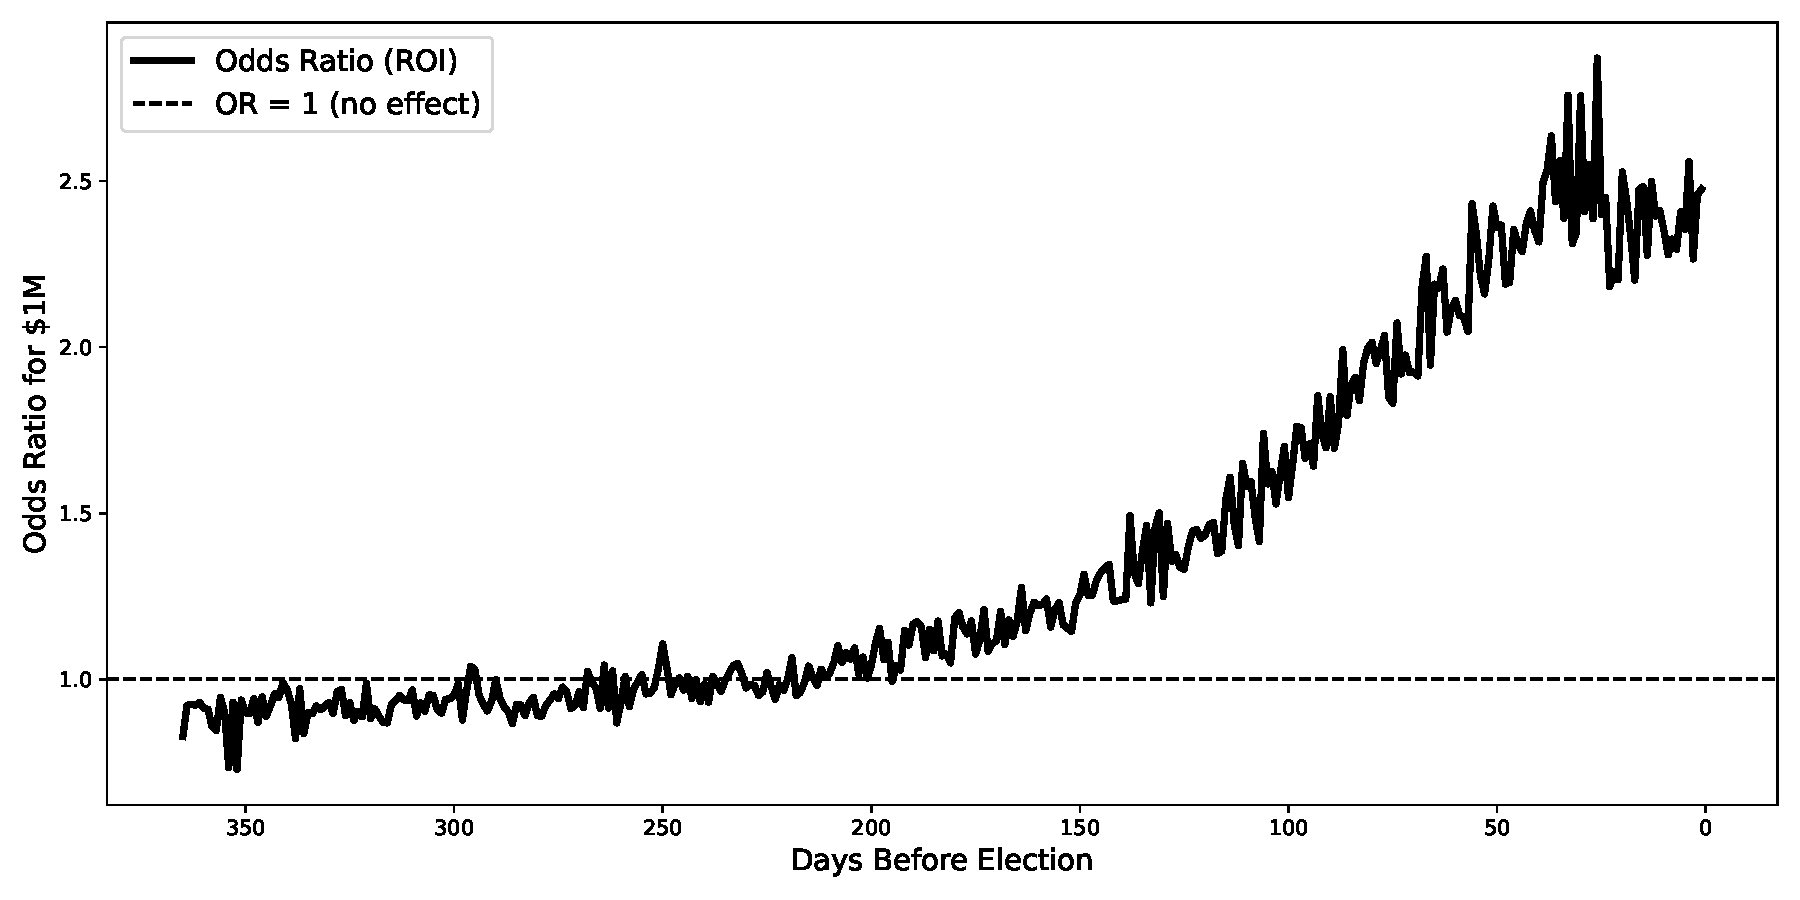
\includegraphics[width = 0.8\linewidth]{../Figures/roi_over_time.pdf}
	\caption{Total Return on Investment Trend over One Year Before Election Day}
	\label{fig:roi-year}
\end{figure}

Additional tables and plots regarding AUC, accuracy, recall, receiver operating characteristic (ROC) curves, and the raw estimated ROI $\beta$ (before converting to an interpretable odds-ratio) are collected in Appendix C.

\subsection*{6.2 Logistic GAM: Win Probability}

Table~\ref{tab:gam-log-roi} summarizes the total ROI estimates for each cutoff $X$ using logistic generalized additive models, and Table~\ref{tab:gam-log-type-roi} shows the by-type ROI estimates in the same manner (\texttt{model\_logisticGAM}). 

\begin{table}[H]
	\centering
	\begin{tabular}{||c c c||}
\hline
Days & Total ROI $\beta$ & Odds-Ratio \\
\hline\hline
360 & -0.285 & 0.752 \\
240 & 0.072 & 1.075 \\
120 & 0.198 & 1.219 \\
60 & -0.107 & 0.898 \\
30 & 0.371 & 1.450 \\
14 & 0.033 & 1.034 \\
7 & 0.308 & 1.360 \\
1 & 0.144 & 1.154 \\
\hline
\end{tabular}

	\caption{GAM Logistic Regression Total ROI Estimates}
	\label{tab:gam-log-roi}
\end{table}

\begin{table}[ht]
	\centering
	\begin{tabular}{||c c c c c c c ||}
\hline
Days & Ind $\beta$ & Ind OR & Comm $\beta$ & Comm OR & Corp $\beta$ & Corp OR \\
\hline\hline
360 & -0.037 & 0.964 & -0.399 & 0.671 & -0.529 & 0.589 \\
240 & 0.471 & 1.602 & -0.111 & 0.895 & -0.275 & 0.759 \\
120 & 0.221 & 1.247 & 0.228 & 1.257 & 0.140 & 1.150 \\
60 & -0.737 & 0.479 & 0.699 & 2.012 & -0.119 & 0.888 \\
30 & 0.039 & 1.040 & 0.320 & 1.377 & 0.868 & 2.382 \\
14 & -0.065 & 0.937 & -0.252 & 0.777 & 0.580 & 1.786 \\
7 & 0.134 & 1.143 & -0.129 & 0.879 & 1.210 & 3.353 \\
1 & 0.058 & 1.060 & -0.445 & 0.641 & 1.178 & 3.249 \\
\hline
\end{tabular}

	\caption{GAM Logistic Regression By-Type ROI Estimates}
	\label{tab:gam-log-type-roi}
\end{table}

Additional metrics, a plot of the ROC curves under this model, and a 365 day trend of the ROI are collected in Appendix C. 

\subsection*{6.3 OLS Regression: Vote Share}

In Table~\ref{tab:lin-roi}, I have collected two ways of expressing estimates of ROI based on least-squares estimates focusing on \$1 million increases in fundraising, the first being the total ROI $\beta$ (the approximation of the change in vote-share percentage points (pp) on the log-scale of dollars), and the latter being the actual marginal effect on vote share (\texttt{model\_linear.py}).

\begin{table}[!t]
	\centering
	\begin{tabular}{||c c c||}
\hline
Days & Total ROI $\beta$ & $\Delta$ \\
\hline\hline
360 & -39.8554 & -8.7519 \\
240 & -22.7274 & -4.9645 \\
120 & -3.1081 & -0.4435 \\
60 & 1.9142 & 0.5872 \\
30 & 5.7872 & 0.8855 \\
14 & 6.0042 & 0.6739 \\
7 & 5.3512 & 0.5154 \\
1 & 6.3002 & 0.6224 \\
\hline
\end{tabular}

	\caption{Linear Regression Raw and Direct ROI}
	\label{tab:lin-roi}
\end{table}

Figure~\ref{fig:feat-importance} depicts the feature importance paths --- absolute standardized coefficents --- for key predictors across cutoffs, while Figure~\ref{fig:heatmap} depicts the heatmap of least-squares $p$-values for selected predictors:

\begin{figure}[H]
	\centering
	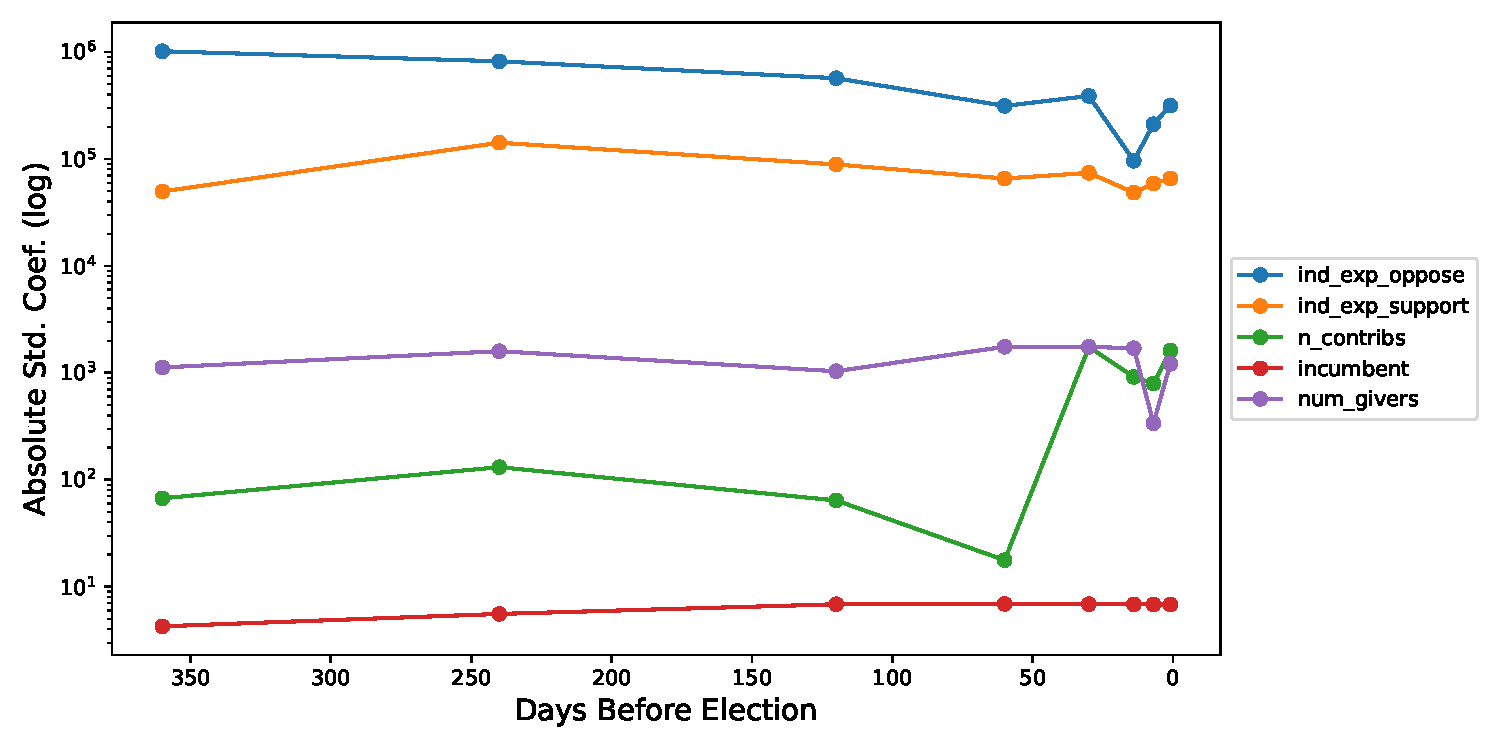
\includegraphics[width = 0.8\linewidth]{../Figures/feat_imp.pdf}
	\caption{Feature Importance Paths across Cutoffs, Logarithmic Scale}
	\label{fig:feat-importance}
\end{figure}

\begin{figure}[H]
	\centering
	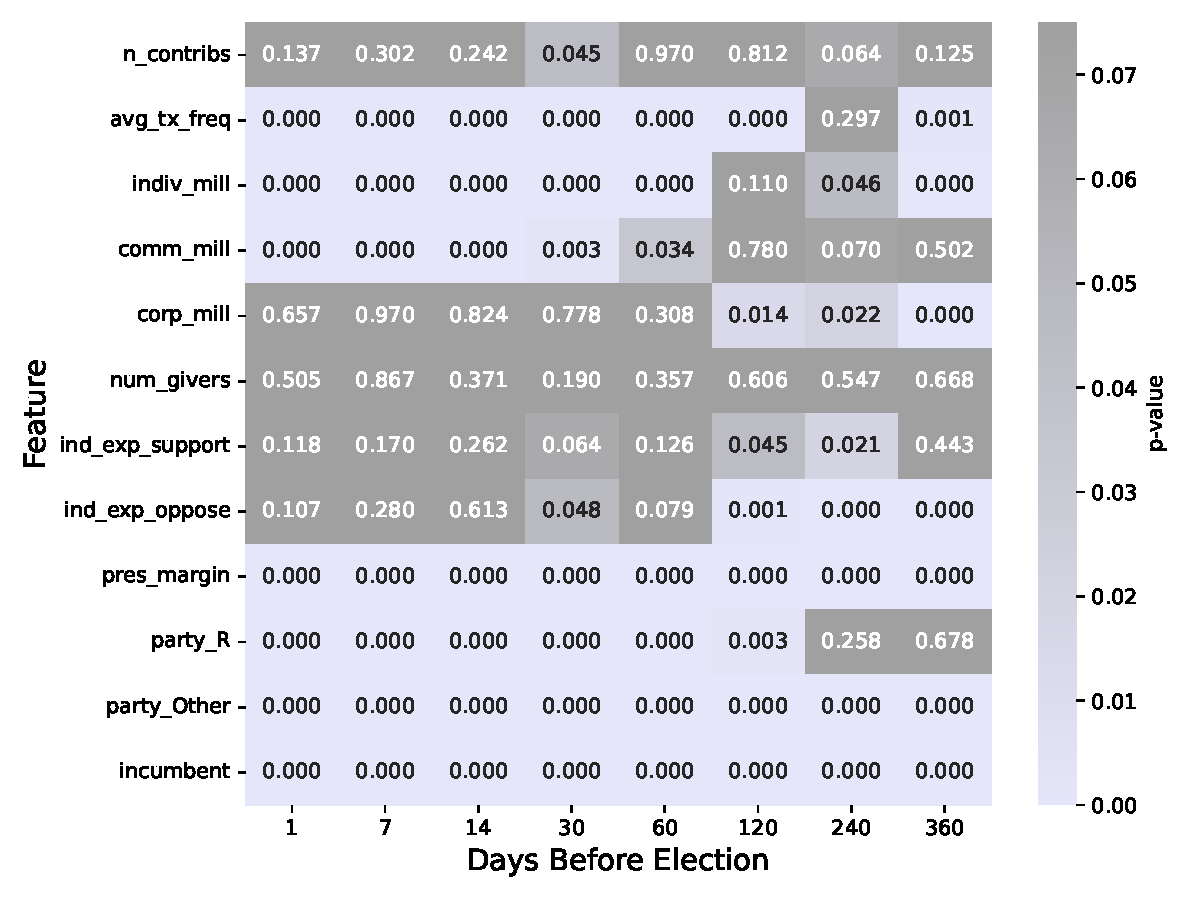
\includegraphics[width = 0.8\linewidth]{../Figures/sig_heatmap.pdf}
	\caption{Least-Squares $p$-value Heatmap for Key Predictors across Cutoffs}
	\label{fig:heatmap}
\end{figure}

Additional information concerning out-of-sample performance metrics ($R^2$, RMSE, MAE), 5-fold CV $R^2$, and regularized $R^2$, and the $\alpha$ used given the better regularization technique (Ridge or LASSO) are collected in Appendix C. 

\subsection*{6.4 Linear GAM: Vote Share}

In Table~\ref{tab:gam-lin-metrics}, I collect the repeated-$k$-fold CV metrics, as well as the GAM ROI-$\Delta$ vote-share (pp) per \$1 million total at the sample-mean mix (\texttt{model\_linearGAM.py}).

\begin{table}[H]
	\centering
	\begin{tabular}{||c c c c c||}
\hline
Days & CV $R^2$ & CV RMSE & CV MAE & $\Delta$ (pp per $1M$) \\
\hline\hline
360 & 0.488 & 12.973 & 8.523 & -1.602 \\
240 & 0.538 & 13.336 & 8.970 & -0.460 \\
120 & 0.502 & 14.837 & 9.377 & 1.741 \\
60 & 0.599 & 13.742 & 9.214 & 2.169 \\
30 & 0.659 & 12.855 & 8.817 & 0.929 \\
14 & 0.680 & 12.514 & 8.693 & -0.193 \\
7 & 0.681 & 12.527 & 8.716 & -0.278 \\
1 & 0.692 & 12.318 & 8.670 & -0.230 \\
\hline
\end{tabular}

	\caption{Linear GAM Cross-Validated Performance by Cutoff}
	\label{tab:gam-lin-metrics}
\end{table}

A supplemental table detailing the hold-out performance at each cutoff is collected in Appendix C.
